%CHAPTER
\chapter{Patent}
%základní informace + uložiště dat + info o zdrojích (patentové úřady atp)
% Nějaká statistika ? graf s počtem patentů od roku 1960+ v Česku, atp.

% chrome-extension://efaidnbmnnnibpcajpcglclefindmkaj/https://www.wipo.int/edocs/pubdocs/en/wipo_pub_941_2021.pdf 
% -> vzít nějakou statistiku

\todo{todo}
Test \cite{InvestopediaPatent, usptoPatent}

\section{Typy patentů}
Patenty jsou klasifikovány do tří hlavních typů: \textbf{Užitný patent}, \textbf{Návrhový patent} a \textbf{Patent rostlin}. V následujících kapitolách jsou tyto typy podrobně popsány a srovnány s jejich právně jednoduššími protějšky.

\subsection{Užitný patent}
Užitný patent, nebo také patent na vynález, poskytuje právní ochranu lidem, kteří vynalézají nový a užitečný proces, výrobní předmět, stroj, složení hmoty nebo užitečné vylepšení. Užitný patent přetrvává 20 let od data podání, pokud jsou placeny udržovací poplatky. Užitné patenty jsou nejběžnějším typem patentů, a lze ho dále rozdělit na 2 podtypy: \textbf{Trvalý} a \textbf{Dočasný}. \cite{usptoUtilityPatent, InvestopediaPatent}.

\subsubsection{Struktura přihlášky užitného patentu} \label{sec:utility_structure}
Struktura užitného patentu obsahuje sedm různých sekcí (v případě \gls{USPTO}), které patent musí obsahovat (pro dočasný patent jsou povinné pouze dvě sekce) \cite{utilityStructure}:
\begin{itemize}
\item \textbf{Pozadí} - Sekce \textbf{Pozadí} popisuje současný stav techniky týkající se navrhovaného vynálezu a neměl by se o tomto vynálezu zmiňovat.\textbf{Pozadí} musí být velmi stručné a nesmí být zveřejněno více informací, než je požadováno.
\item \textbf{Stručný přehled} - Sekce \textbf{Stručný přehled} shrňuje oddíl \textbf{Podrobný popis} do několika odstavců.
\item \textbf{Stručný popis nákresů} - Sekce \textbf{Stručný popis nákresů} obsahuje široký přehled nákresů v oddílu \textbf{Nákresy}. Lze zde zmínit a identifikovat části vynálezu v každém z obrázků nebo například uvádět rúzné pohledy nákresů (perspektivní, pohled zleva a zprava, ...).
\item \textbf{Podrobný popis} - Sekce \textbf{Podrobný popis} popisuje různá alternativní provedení a vlastnosti vynálezu a měla by obsahovat referenční číslice, které odkazují na obrázky v oddílu \textbf{Nákresy}. Tato je povinná i pro dočasnou přihlášku.
\item \textbf{Nároky} - Sekce \textbf{Nároky} popisuje rozsah ochrany poskytované patentem nebo ochranu požadovanou v patentové přihlášce.
\item \textbf{Abstrakt} - Sekce \textbf{Abstrakt} slouží jako krátké shrnutí o čem patent je. Abstrakt nesmí být delší jak 150 slov.
\item \textbf{Nákresy} - Sekce \textbf{Nákresy} obsahují nákresy popisující vlastnosti vynálezu v různých náhledech (perspektivní, ...).  Tato je povinná i pro dočasnou přihlášku.
\end{itemize}

\subsubsection{Užitný patent vs Užitný vzor}
Patentová ochrana neníí jedinou formou průmyslově právní ochrany vynálezu. Pro vynálezy s nižší vynálezeckou úrovní je možné zvolit \textbf{Užitný vzor}, který je jednodušší, rychlejší a méně nákladnou alternativou k užitnému patentu.

\subsection{Návrhový patent}
Návrhový patent, jinak zvaný jako Průmyslový vzor, je patent vydaný pro originální, nové a ornamentální vzory pro vyráběné výrobky. Vzhledem k tomu, že se návrhový patent projevuje vzhledem, atk se předmět patentové přihlášky může týkat konfigurace nebo tvaru předmětu, povrchové výzdoby aplikované na předmět nebo kombinace konfigurace a povrchové výzdoby. Návrh povrchové výzdoby je neoddělitelný od předmětu, na který je aplikován, a nemůže existovat sám. Lze získat návrhový i užitný patent na jeden produkt v případě, že z technologického a designového hlediska jsou neoddělitené. Návrhový patent má platnost (stejně jako u ostatních patentů) od 5 až do 25 let (každá země může mít jinak nastavenou platnost) \cite{usptoDesignPatent}.

\subsubsection{Struktura přihlášky návrhového patentu}
Struktura přihlášky návrhového patentu by měla obsahovat tyto prvky (v případě \gls{USPTO}):
\begin{itemize}
\item Preambule s uvedením jména přihlašovatele, názvu návrhového patentu a strušného popisu použití předmětu, ve kterém je tento návrh ztělesněn.
\item Křížový odkaz na související užitkovou žádost.
\item Prohlášení týkající se federálně sponzorovaného výzkumu nebo vývoje.
\item Popis obrázků a výkresů.
\item Popis funkce.
\item Jeden nárok na návrh.
\item Výkresy a fotografie.
\item Vykonaný slib nebo přísaha.
\end{itemize}

\subsubsection{Návrhový patent vs Ochranná známka}
Ochranná známka je označení pro schopné grafické znázornění, tvořené zejména slovy, písmeny, číslicemi, barvou, kresbou nebo tvarem výrobku či jeho obalu, určené k rozlišení výrobků nebo služeb\cite{ceskoOchranna}, zatímco návrhový patent se vztahuje na okrasný vzhled výrobku jako takového, který není spojen s identifikací zdroje zboží \cite{designTrademark}.

\subsection{Patent rostlin}
Patent na rostlinu je vydáván na novou nebo odlišnou odrůdu rostliny, která byla vynalezena nebo objevena a asexuálně rozmnožována. Tyto patenty se udělují na 20 let od data podání přihlášky a neplatí se žádné udržovací poplatky \cite{usptoPlantPatent}. Účelem těchto patentů je zamezení duplikování rostlin nebo jejich nabízení k prodeji (jako celek nebo po částech).
\subsubsection{Struktura přihlášky patentu rostlin}
Struktura patentu pro rostliny (v případě \gls{USPTO}) je až jednu vyjímku stejná jako pro užitný patent (viz kapitola č. \ref{sec:utility_structure}). Vyjímka se týká podrobného popisu, který musí obsahovat kompletní botanický popis dané rostliny a rozdíly, které tuto rostlinu odlišují od ostatních, již existujích rostlin.

\section{Přihláška vs Publikace}
% popsat rozdíly, případně nějaká tabulka atp.
%There are two types of utility and plant patent applications: provisional and nonprovisional.

\todo{todo}

\section{Obory}
Každý patent je po podání přihlášky klasifikován do jednoho oboru podle klasifikačního systému \gls{IPC}. \textbf{International Patent Classification} (\gls{IPC}) je hierarchický systém, který používá jazykově nezávislé symboly pro klasifikaci patentů a užitných vzorů podle oblasti technologie, ke které se vztahují \cite{espacenetIPC}. Tento systém je používán ve více než 100 zemí. 
\newline
\indent \gls{IPC} schéma definuje celkem osm hlavních oblastí technologie, do kterých lze patent přiřadit. Každá oblast je symbolizována jedním písmenem (viz tabulka č. \ref{tab:kind_codes}).

	\begin{table}[H]
	\centering
	\begin{tabular}{|>{\centering\arraybackslash}p{1cm}|>{\centering\arraybackslash}p{12cm}|}
	\hline
	\textbf{Kód}    & \textbf{Popisek}\\
	\hline
	A & Lidské potřeby - jídlo, léky, oblečení, ... \\
	\hline
	B & Operace a Doprava - tisk, auta, koleje, nanotechnologie, ...\\
	\hline
	C & Chemie a Hutnictví - sklo, cement, železo, ...\\
	\hline
	D & Textílie a Papír - výroba papíru, provazy, tkalcovství \\
	\hline
	E & Pevné konstrukce -  stavby, dveře, zámky, dolování, ... \\
	\hline
	F & Strojírenství, Osvětlení, Vytápění, Zbraně, Odstřelování \\
	\hline
	G & Fyzika -  měření, testování, optika, nukleární fyzika, ...\\
	\hline
	H & Elektřina - zákadní elektrické elementy (kabely, rezistory, ...), techniky elektrické komunikace, ...  \\
	\hline
	\end{tabular}
	\caption{Základní \gls{IPC} klasifikace oborů \cite{ipc_class}.}
	\label{tab:kind_codes}
	\end{table}

\noindent Klasifikační symboly definované \gls{IPC} jsou tvořeny písmenem označující hlavní oblast technologie (neboli sekce), následovaným dvěmi číslicemi označující třídu, poté písmenem označujícím podtřídu. Po podtřídě následuje proměnná čítající jednu až čtyří číslice, která označuje hlavní skupinu. Následuje dopředné lomítko a číslo čítající dvě až šest číslic označující podskupinu \cite{espacenetIPC}. Příklad klasifikace lze vidět v tabulce č. \ref{tab:ipc_example}.

	\begin{table}[H]
	\centering
	\begin{tabular}{|>{\centering\arraybackslash}p{2cm}|>{\centering\arraybackslash}p{2cm}|>{\centering\arraybackslash}p{2.5cm}|>{\centering\arraybackslash}p{6cm}|}
	\hline
	\textbf{Divize}    & \textbf{Počet divizí} & \textbf{Symbol} & \textbf{Titulek} \\
	\hline
	Sekce & 8 & G & Fyzika \\
	\hline
	Třída & 120 & G01 & Měření; Testování \\
	\hline
	Podtřída & 628 & G01G & Vážení \\
	\hline
	Skupina & +- 6 900 & G01G 21 & Podrobnosti o vážení aparátu \\
	\hline
	Podskupina & +- 62 100 & G01G 21/02 & Podrobnosti o vážení ložisek s ostřím nože   \\
	\hline
	\end{tabular}
	\caption{Příklad \gls{IPC} klasifikace \cite{ipcTable}.}
	\label{tab:ipc_example}
	\end{table}

%%%%%%%%%%%%%%%%%%%%%%%%%%%%%%%%%%%%%%%%%%%%%%%%%%%%%%%%%%%%

%CHAPTER
\chapter{Databáze} \label{chap:databaze}

Termín databáze označuje organizovanou kolekci strukturovaných informací nebo dat, která jsou typicky ukládána elektronicky v počítačovém systému. Data / informace lze nazvat jako fakta vztahující se k libovolnému uvažovanému objektu. Typický příklad objektu je člověk, jehož fakta jsou: jméno, věk, výška, váha a mnoho dalších \cite{guru99Database}.\newline

\section{Systém řízení báze dat}
Pro správu dat v databázi a její řízení je potřeba komplexní software, který se nazývá \textbf{Systém Řízení Báze Dat} (SŘBD, anglicky \gls{DBMS}). SŘBD slouží jako interface mezi samotnou databází a koncovým uživatelem (může být i program), umožňující jak vytěžování a aktualizaci dat, tak i možnosti nastavení záloh a jiných administrativních operací \cite{OracleDB}. V dnešním světe existuje několik různých \gls{DBMS} (například Relační \gls{DBMS}, Objektově-orientované \gls{DBMS}).
\begin{figure}[h!]
\centering
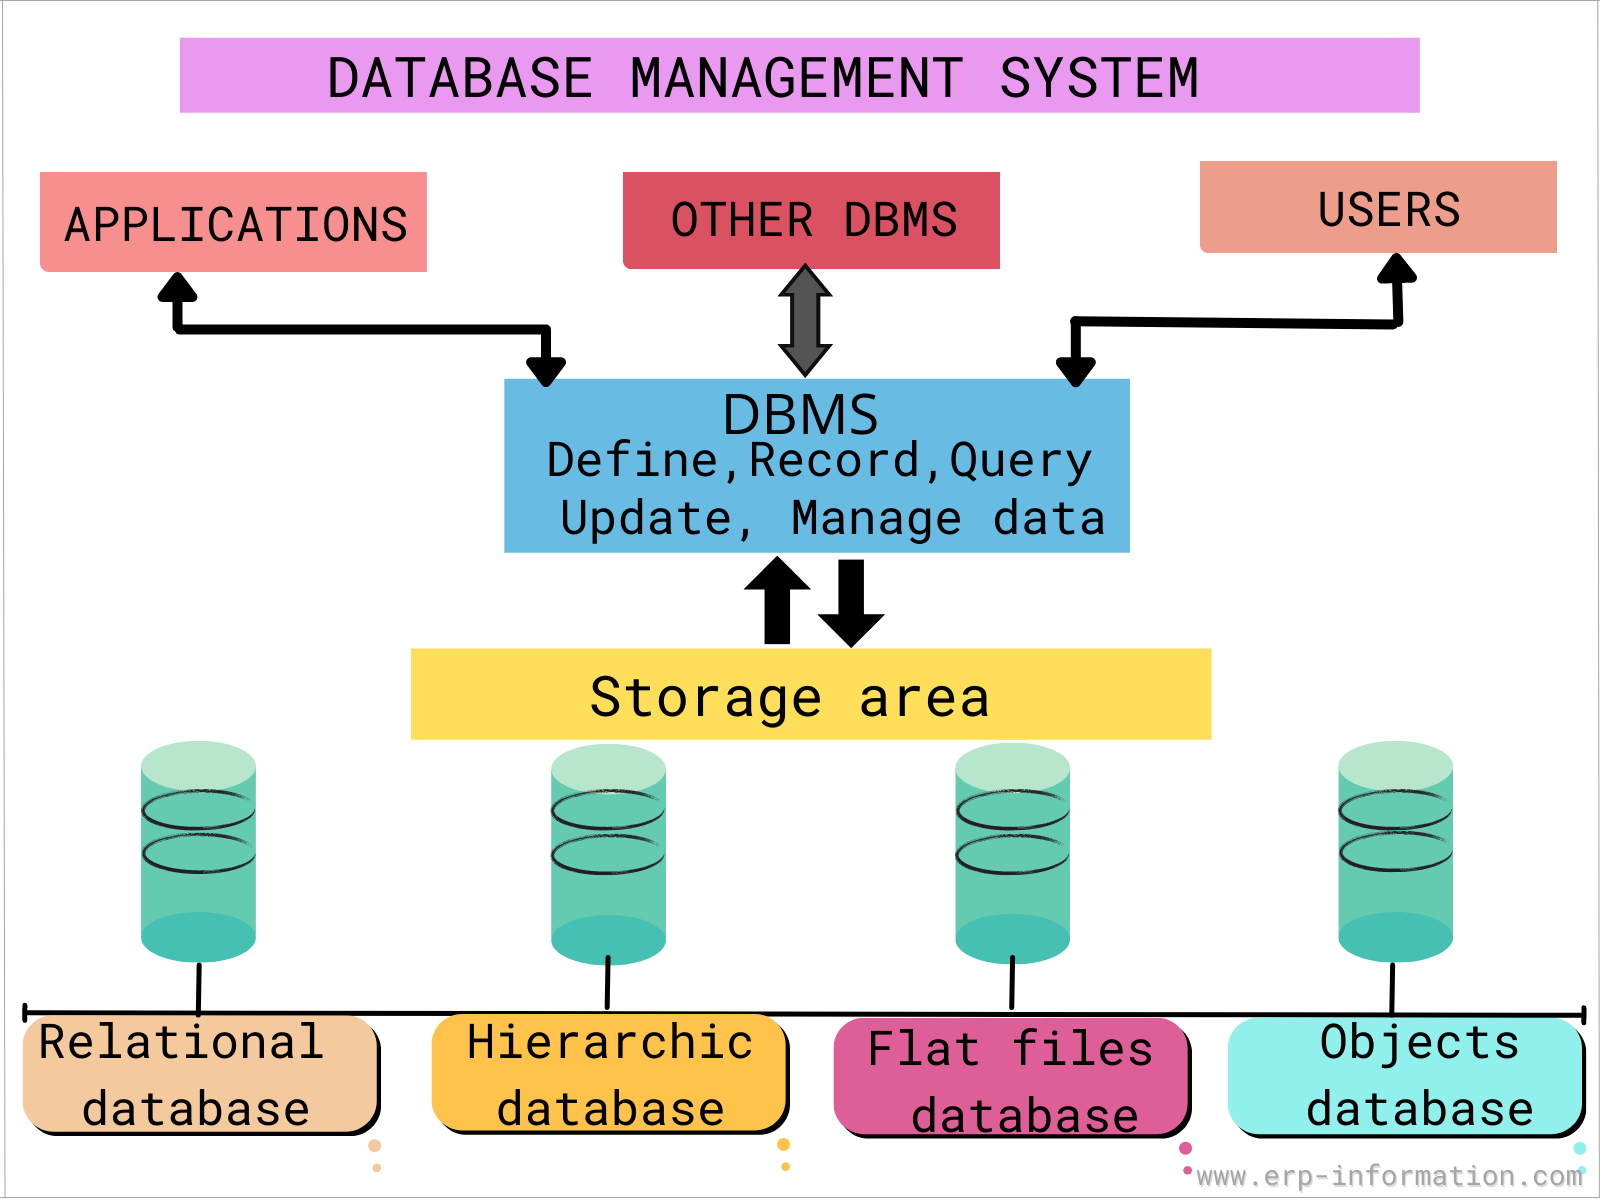
\includegraphics[width=10cm]{img/databaze/dbms}
\caption{Systém řízení báze dat \cite{img_dbms}.}
\label{fig:dbms}
\end{figure}

\section{Komponenty databáze}
Všechny databáze sestávají z pěti základních komponent, nehledě na použitý typ databáze \cite{TechTargetDB, guru99Database}:
\begin{itemize}
\item \textbf{Hardware} - Fyzické stroje (počítače, servery, pevné disky, ...) na kterých běží databázový software.
\item \textbf{Software} - Databázový software poskytuje uživateli / programu kontrolu nad databází. Zahrnuje to samotný databázový software, operační systém, software pro správu sdílení dat mezi uživately a programy pro přístup k datům v databázi.
\item \textbf{Data} - Nezpracované a neorganizované fakty, které je potřeba zpracovat. Administrátor databáze organizuje tyto data a dává jim význam. Data se obecně skládají hlavně z faktů, observací, percepcí, čísel, znaků a mnoho dalších.
\item \textbf{Jazyk} - Typický příklad použití jazyku je přístup k datům, přidávání nových dat, úpravu již existujících dat z databáze. Uživatel / program napíše specifické příkazy v jazyku pro přístup k datům (Database Access Language) a tyto příkazy následně pošle databázi ke zpracování. Více viz kapitola č. \ref{sec:jazyky}.
\item \textbf{Procedury} - Procedura obsahuje předpřipravený seznam příkazů, které se následně vykonávají po zavolání dané procedury. 
\end{itemize}

\section{Typy databází} \label{sec:typy_databazi}
V dnešním světě existuje mnoho různých typů databází. Výběr nejlepšího typu databáze pro konkrétní organizaci závisí na tom, jak organizace zamýšlí data používat. V této kapitole je vypsáno pouze pár typů, protože vznikají stále nové, méně známé typy databází, které jsou tvořeny pro specifické požadavky (například finanční, věděcké) \cite{matillionTypeDB, OracleDB}.

\subsection{Relační databáze}
Název relační databáze pochází ze způsobu, jakým jsou data uložena, a to ve více souvisejících tabulkách. Data v tabulkách jsou uložena v řádcích a sloupcích. Relační databáze jsou velice spolehlivé a podporují všechny čtyři žádoucí vlastnosti databázových transakcí \gls{ACID}. Pro co nejefektivěnjší využití tohoto typu databáze je potřeba ukládat pouze dobře strukturovaná data, pro částečně strukturovaná či nestrukturovaná data je vhodné použít například grafové nebo dokumentově založené databáze. Typické relační databáze jsou například: Microsoft SQL Server, Oracle Database, MySQL. Ukázku relační databáze lze vidět na obrázku č. \ref{fig:db_img_relational}.
	\begin{figure}[H]
	\centering
	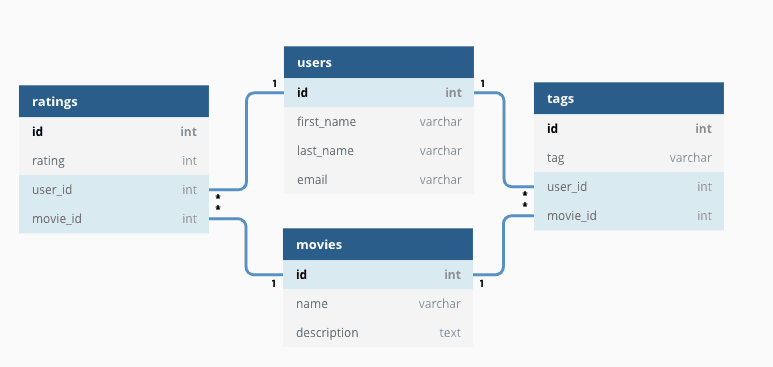
\includegraphics[width=14cm]{img/databaze/relational_db}
	\caption{Ukázka relační databáze.}
	\label{fig:db_img_relational}
	\end{figure}
\subsubsection{Datový model}
Relační datový model obsahuje několik fundamentálních konceptů. Koncepty lze vidět na obrázku č. \ref{fig:model_relational}.
\begin{figure}[H]
\centering
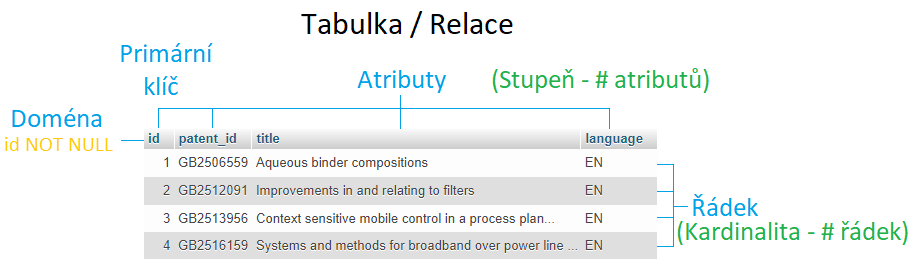
\includegraphics[width=16cm]{img/databaze/data_model_relational}
\caption{Koncepty relačního datového modelu \cite{data_model_oo}.}
\label{fig:model_relational}
\end{figure}

\indent První z konceptů se nazývá \textbf{Relace}, což je dvou-dimenzionální tabulka, která se používá pro ukládání kolekce datových elementů. Tabulka je tvořena řádky a sloupci, kde řádky reprezentují záznamy a sloupce reprezentují atributy.
\newline
\indent \textbf{Řádka} je další koncept relačního modelu, která pouze reprezentuje jeden záznam v tabulce.
\newline
\indent Další z konceptů je \textbf{Atribut}, který reprezentuje sloupec v tabulce, neboli vlastnosti jednotlivých řádků (například jméno, příjmení, věk, ...).
\newline
\indent Koncept \textbf{Doména atributů} slouží k definici vlastností pro každou hodnotu daného atributu. Pomocí domény lze určit, zda hodnoty daného atributu mohou být prázdné, budou dlouhé maximálně 50 znaků nebo například určit datový typ atributu (textová hodnota, číslo, ...).
\newline
\indent Další z konceptů je \textbf{Stupeň}, který pouze určuje počet atributů v dané relaci.
\newline
\indent \textbf{Kardinalita} určuje počet řádků / záznamů existujících v dané relaci.
\newline
\indent Koncept \textbf{Relační schéma} popisuje návrh a strukturu relace. Obsahuje názvy tabulek, jejich atributy a typy atributů. Relační schéma pro naší tabulku lze vidět na obrázku č. \ref{fig:schema_relation}.
\begin{figure}[H]
\centering
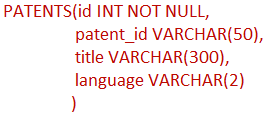
\includegraphics[width=6cm]{img/databaze/schema_relation}
\caption{Relační schéma pro tabulku na obrázku č. \ref{fig:model_relational}.}
\label{fig:schema_relation}
\end{figure}

\indent \textbf{Relační instance} reprezentuje kolekci záznamů, které jsou uložené v tabulce v určitém čase.
\newline
\indent Poslední koncept \textbf{Relační klíč} je atribut / seznam atributů, které lze využít jako unikátní identifikátor jedné entity v tabulce, případně k určení vazby mezi dvěma relacema. Existuje šest typů relačních klíčů - kandidátní, super, složený, primární, cizí, sekundární / alternativní \cite{data_model_relation}.

\subsubsection{Výhody}
Výhody relační databáze jsou \cite{advantages_relational}:
\begin{itemize}
\item \textbf{Jednoduchost modelu} - Při porovnávání ostatních typů databází s relačním, relační databáze je o mnoho jednodušší. Díky tomu, že zde neprobíhá žádné zpracování dat, tak není potřeba využívat žádné složité dotazy.
\item \textbf{Snadné použití} - Uživatelé můžou jednoduše přistupovat a získávat všechny potřebné informace v rámci sekund bez ohledu na složitost databáze.
\item \textbf{Přesnost} - Relační databáze jsou dobře uspořádané a velice striktně definované. I za pomoci primárních a cizích klíčů se v databázi udržuje unikátnost hodnot, takže se zde nevyskytují žádné duplikáty.
\item \textbf{Integrita dat} - Integrita dat zajišťuje konzistentnost všech tabulek v databázi, díky čemuž lze dosáhnout vlastností jako přesnost a snadné použití.
\item \textbf{Normalizace} - Normalizace je metoda, pomocí které lze rozdělit jednu informaci do několika bloků za účelem snížení velikosti.
\item \textbf{Spolupráce} - Více uživatelů může přistupovat k datům ve stejný čas i v případě, že část dat je upravována.
\item \textbf{Bezpečnost} - Bezpečnost je zajištěna autorizací uživatelů, kdy pouze uživatelé s právy a přístupovými údaji mohou přistupovat k datům.
\end{itemize}
\subsubsection{Nevýhody}
Nevýhody relační databáze jsou \cite{advantages_relational}:
\begin{itemize}
\item \textbf{Problém s údržbou} -  Údržba relační databáze se stává postupem času náročnější vzhledem ke zvýšenému počtu uložených dat.
\item \textbf{Cena} - Systém relační databáze je drahý k pořízení i pro správu. Samotná prvotní cena systému je relativně drahá pro menší byznys, ale zhoršuje se při zohlednění najímání profesionálních techniků, které musí mít dobré znalosti ohledně používaného systému.
\item \textbf{Fyzické úložiště} - Relační databáze jsou složeny z řádků a sloupců, které potřebují hodně fyzické paměti, protože každá provedená operace závisí na samostatném úložišti. 
\item \textbf{Malá škálovatelnost} - Při používání relační databáze na více serverech se její struktura mění a stává se obtížně zvládnutelnou, zejména při velkém objemu dat. Jak se databáze zvětšuje nebo více distribuuje s větším počtem serverů, tak se zvětšuje latence a problémy s dostupností, které ovlivňují celkový výkon.
\item \textbf{Složitost struktury} - Relační databáze dokáží ukládat data pouze v tabulkové formě, která neumožňuje vyobrazit složitější vazby mezi objekty. Toto může být velký problém u dost aplikací, u kterých data nelze reprezentovat pouze jednou tabulkou díky jejich aplikační logice.
\item \textbf{Snížení výkonu postupem času} - S větším množstvím uložených dat a tabulek se zvětšuje i složitost systému, díky čemuž bude systém reagovat pomaleji na dotazy, případně může i spadnout v případě více dotazů od více uživatelů.
\end{itemize}

\subsection{Objektově-orientovaná databáze}
Objektově-orientovaná databáze je založena na objektově-orientovaném programování, kdy data a všechny jejich atributy a metody jsou svázány dohromady jako objekt. Stejně jako relační databáze, i objektově-orientované databáze odpovídají standardům \gls{ACID}. Typické příklady jsou například: ObjectStore, ConceptBase. Ukázku objektově-orientované databáze lze vidět na obrázku č. \ref{fig:db_img_oo}.
	\begin{figure}[H]
	\centering
	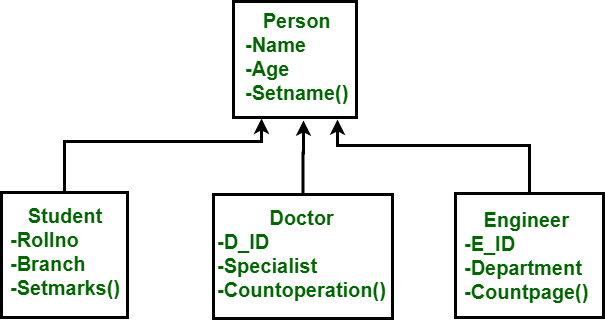
\includegraphics[width=11cm]{img/databaze/oo_db}
	\caption{Ukázka objektově-orientované databáze.}
	\label{fig:db_img_oo}
	\end{figure}
\subsubsection{Datový model}
V objektově-orientovaném modelu jsou data a jejich vztahy mezi sebou uložené v jediné struktuře, která se jinak nazývá objekt. Všechny objekty mají mezi sebou vícenásobné vztahy. Jednoduše řečeno, objektově-orientovaný datový model je spojením relačního databázového modelu a objektově-orientovaného programování \cite{data_model_oo}.
\newline
\noindent V datovém modelu existují tyto komponenty:
\begin{itemize}
\item \textbf{Objekt} - Objekt je abstrakcí jakékoliv entity z reálného světa, jinak zvaná jako instance jedné třídy. Objekt zapouzdřuje data a funkční kód do celku, který poskytuje pouze datovou abstrakci, zatímco schovává implementační detaily od uživatele. Příklad objektů z obrázku č. \ref{fig:db_img_oo}: \textit{Student}, \textit{Doktor} a \textit{Inženýr} jsou instancí celku \textit{Člověk}.
\item \textbf{Atribut} - Atribut popisuje vlastnosti objektu. Například \textit{Student} obsahuje atributy \textit{Číslo} a \textit{Obor}.
\item \textbf{Metoda} - Metoda reprezentuje chování objektu. Například \textit{Student} obsahuje metodu s názvem \textit{nastav\_obor}, pomocí které můžeme získat studovaný obor daného studenta.
\item \textbf{Třída} - Třída je vlastně kolekce podobných objektů, které sdílejí strukturu (neboli atributy) a chování (neboli metody). 
\item \textbf{Dědičnost} - Vytvořenému objektu se říká instance třídy, která zdědí kopie / instance všech atributů a metod dané třídy. \textit{Student}, \textit{Doktor} i \textit{Inženýr} dědí od celku \textit{Člověk} atributy \textit{Jméno}, \textit{Věk} a metodu \textit{nastav\_jmeno}.
\end{itemize}

\subsubsection{Výhody}
Výhody objektově-orientované databáze jsou \cite{advantages_oo}:
\begin{itemize}
\item \textbf{Výkonnost} - Mnohonásobně výkonnější než relační databáze.
\item \textbf{Rozšiřitelnost} - lze vytvářet nové datové typy z již existujících. Jako příklad lze uvést vytvořením super třídy, která bude obsahovat všechny společné atributy a metody. Tímto lze snížit redundanci v systému.
\item \textbf{Podpora velkého množství datových typů} - Oproti ostatním typům databáze, objektově-orientovaná databáze podporuje ukládání různých typů dat, jako například obrázky, zvuky, video a mnoho dalších.
\item \textbf{Podpora vývoje schématu} - Těsné propojení mezi daty a aplikacemi činí vývoj schématu více proveditelnějším.
\item \textbf{Podpora pro dlouhotrvající transakce} - Objektově-orientovaná databáze využívá jiný protokol pro zpracovávání dlouhotrvajících transakcí než relační databáze.
\end{itemize}

\subsubsection{Nevýhody}
Nevýhody objektově-orientované databáze jsou \cite{advantages_oo}:
\begin{itemize}
\item \textbf{Neexistující univerzální datový model} - V dnešní době stále neexistuje univerzální datový model, navíc většině modelů chybí teoretický základ.
\item \textbf{Nedostačující standardy} - Pro objektově-orientované databáze neexistují žádný univerzální datový model, stejně jako standardní dotazovací jazyk.
\item \textbf{Složitost} - Funkcionality jako například dlouhotrvající transakce, zpráva verzí nebo evoluce schémat činí výsledný systém mnohonásobně složitější, což vede k vyšší ceně a složitějšímu používání.
\item \textbf{Zabezpečení} - V databázi neexistuje adekvátní zabezpečovací systém, který by mohl přiřazovat přístupová práva na objekty nebo třídy.
\end{itemize}

\subsection{NoSQL databáze}
NoSQL je široká kategorie databází, které nepoužívají \gls{SQL} jako svůj primární jazyk pro přístup k datům. Tyto typy databází jsou také někdy označovány jako nerelační databáze. V NoSQL databázích se pracuje s nestrukturovanými a polostrukturovanými sadami distribuovaných dat. Jednou z výhod je, že vývojáři mohou provádět změny databáze za běhu, aniž by to ovlivnilo aplikace, které databázi používají.

\subsection{Databáze Klíč-Hodnota}
Databáze klíč-hodnota poskytuje nejjednodušší možný NoSQL datový model. Data jsou uložená jako pár klíč - hodnota ve slovníku / mapě, kdy klíč je indexem. Hodnota může být například celé číslo, řetězec, struktura \gls{JSON} nebo pole. Z vlastností databáze vyplývá, že zde není potřeba žádný dotazovací jazyk pro získávání výsledků. Typické příklady jsou: Redis, Riak, LevelDB. Ukázku databáze klíč-hodnota lze vidět na obrázku č. \ref{fig:db_img_keyvalue}.
	\begin{figure}[H]
	\centering
	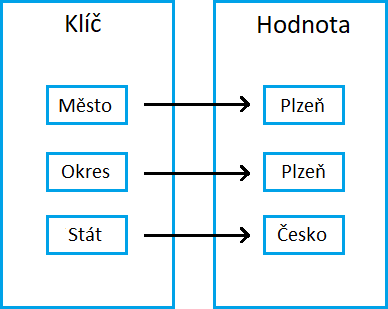
\includegraphics[width=9cm]{img/databaze/keyvalue_db}
	\caption{Ukázka databáze klíč-hodnota.}
	\label{fig:db_img_keyvalue}
	\end{figure}
\subsubsection{Výhody}
Výhody této databáze jsou \cite{advantages_keyvalue}:
\begin{itemize}
\item \textbf{Škálovatelnost} - Databázi lze škálovat jak vertikálně, tak i horizontálně. 
\item \textbf{Redundance} - Zabudovaná redundance zapříčiňuje větší spolehlivost databáze.
\item \textbf{Rychlost} - Reakční čas je velice rychlý díky jednoduchosti struktury a jednoduchých příkazů (vlož, smaž, získej).
\end{itemize}

\subsubsection{Nevýhody}
Nevýhody této databáze jsou \cite{advantages_keyvalue}:
\begin{itemize}
\item \textbf{Optimalizace dat} - Optimalizace je provedena pouze pro data, kde je pouze jeden klíč a jedna hodnota. V případě ukládání složitějších struktur je potřeba parser. 
\item \textbf{Složité dotazy} - Nelze používat složité dotazy, pomocí kterých lze vyhledávat specifické hodnoty.
\end{itemize}

\subsection{Grafová databáze}
Grafová databáze je typem NoSQL databáze, která je založená na teorii grafů. Data jsou reprezentována jako uzly, hrany zase reprezentují vztahy mezi daty. Graf lze procházet podél určitých typů hran nebo přes celý graf. Procházení spojení nebo relací je velmi rychlé, protože vztahy mezi uzly se nepočítají v době dotazu, ale jsou v databázi trvalé. Typické příklady jsou: Neo4j, OrientDB, Microsoft Azure CosmosDB. Ukázku grafové databáze lze vidět na obrázku č. \ref{fig:db_img_graph}.
	\begin{figure}[H]
	\centering
	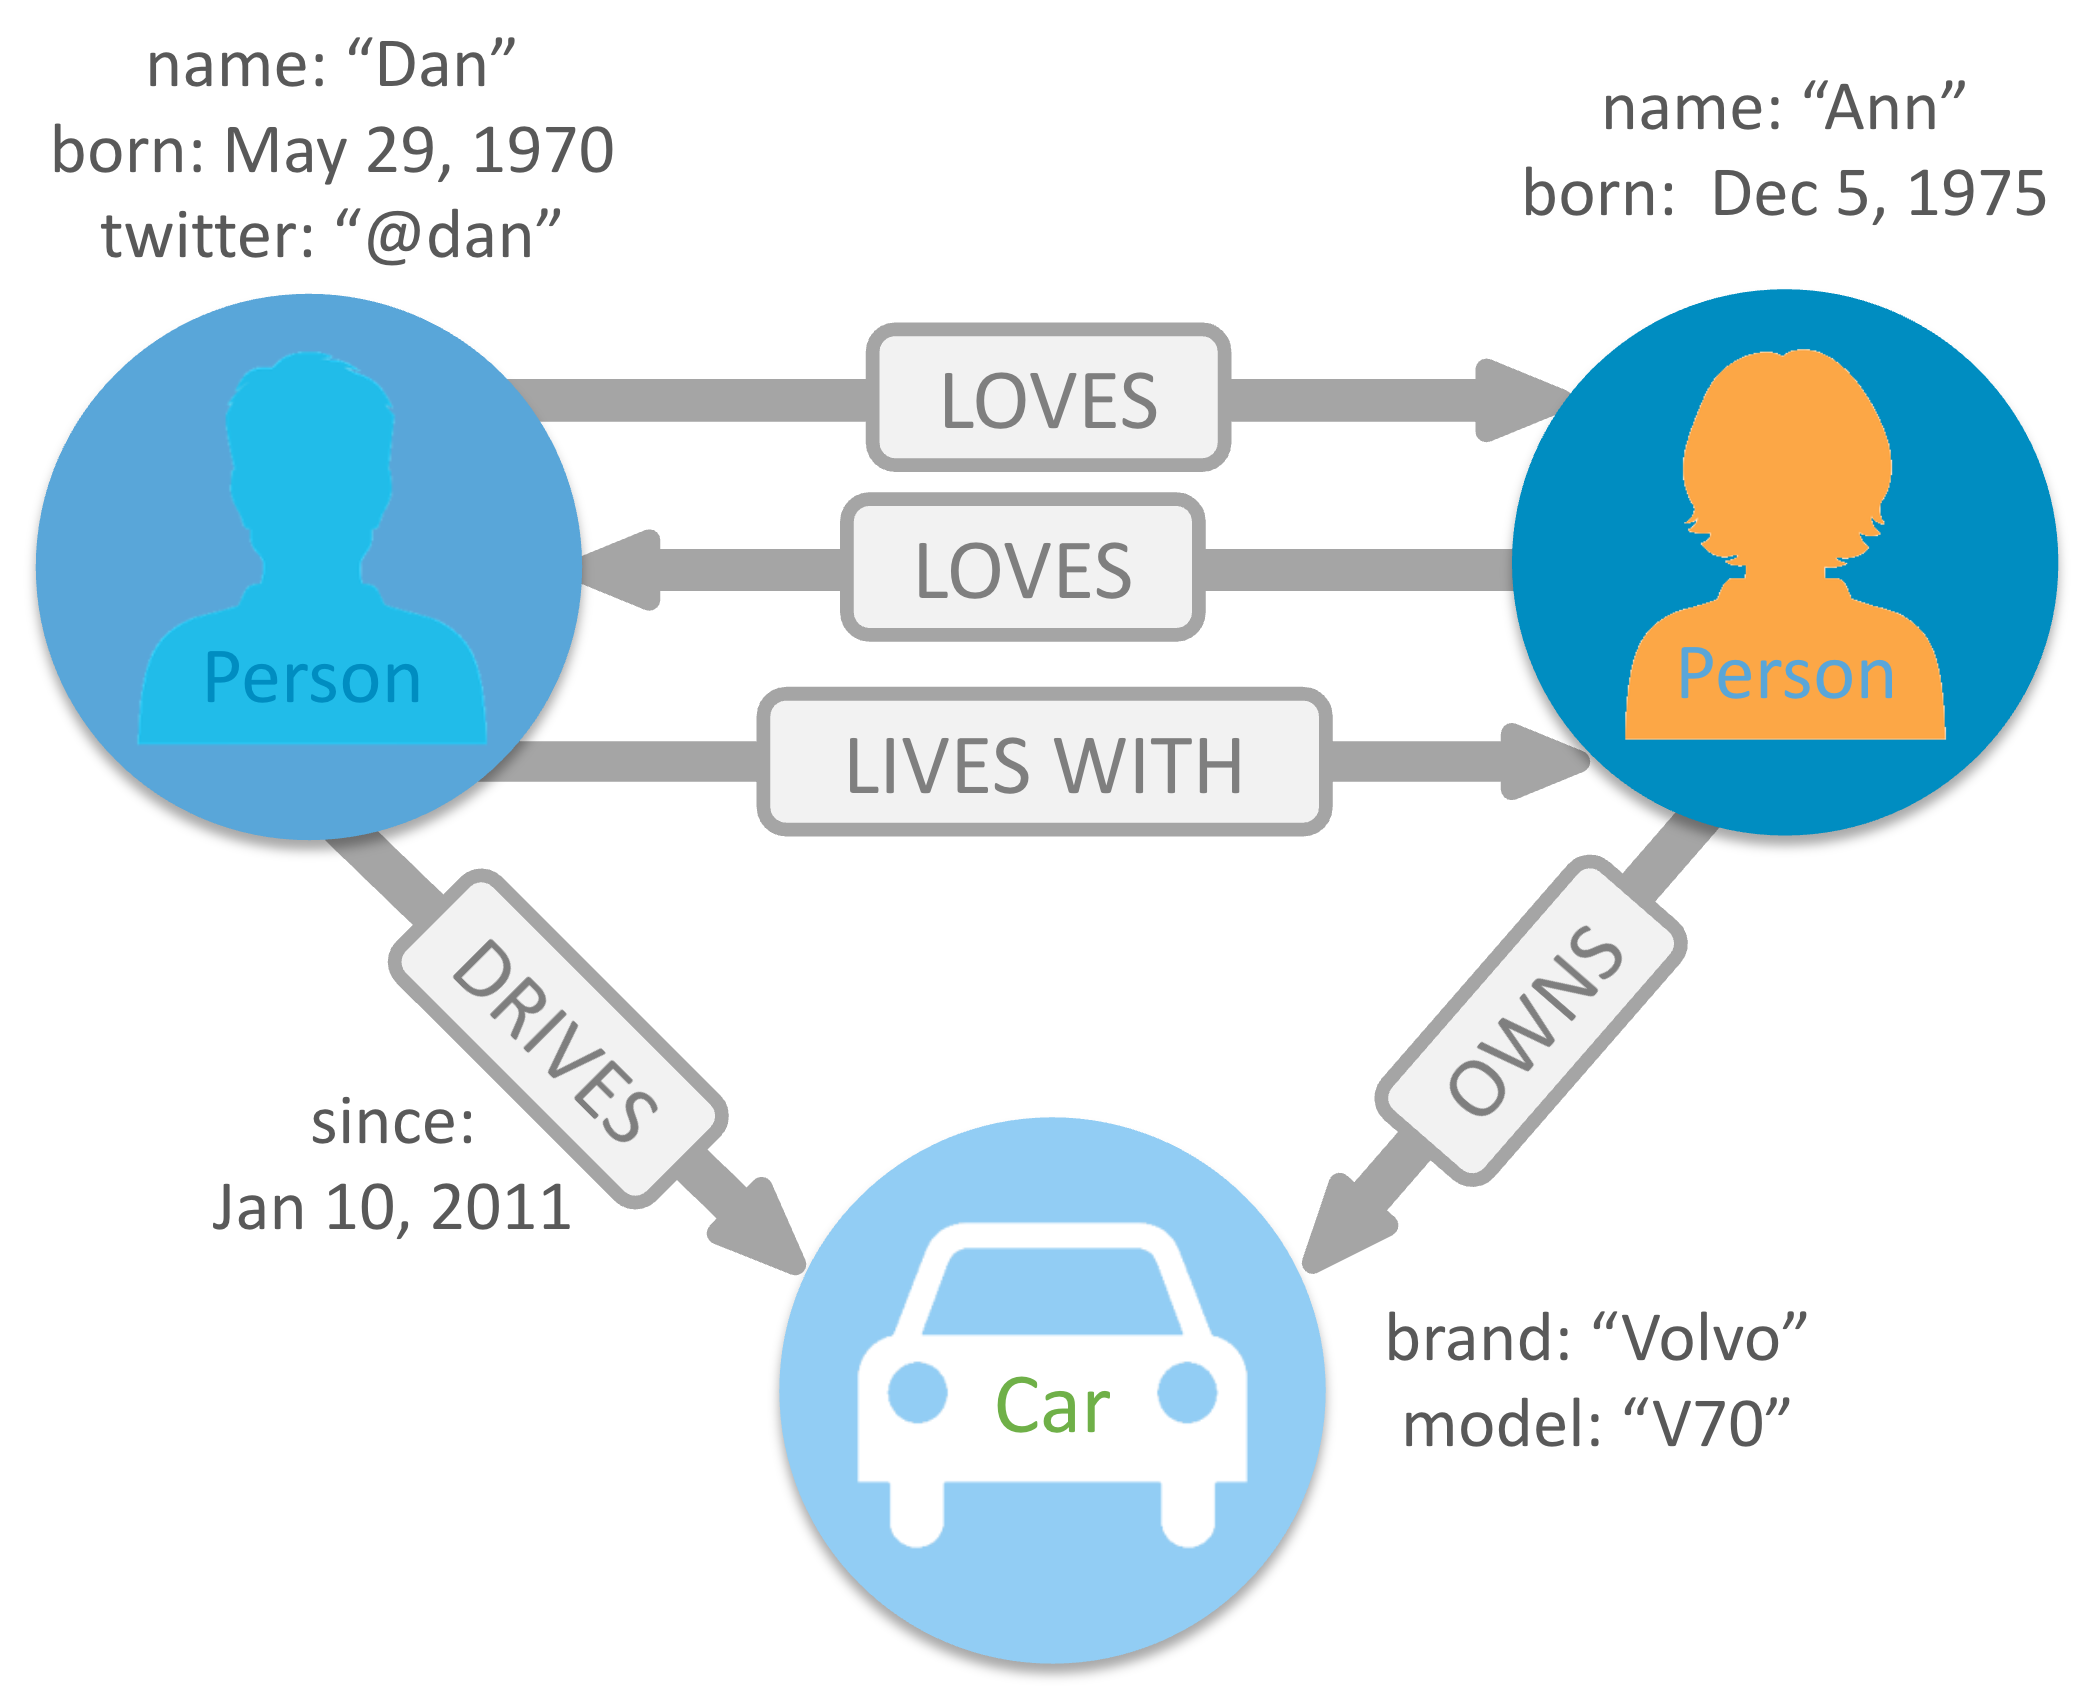
\includegraphics[width=8cm]{img/databaze/graph_db}
	\caption{Ukázka grafové databáze \cite{neo_graph}.}
	\label{fig:db_img_graph}
	\end{figure}
\subsubsection{Datový model}
Datový model grafové databáze se skládá ze čtyř komponent (viz obrázek č. \ref{fig:graph_components}) \cite{data_model_graph}:
	\begin{figure}[H]
	\centering
	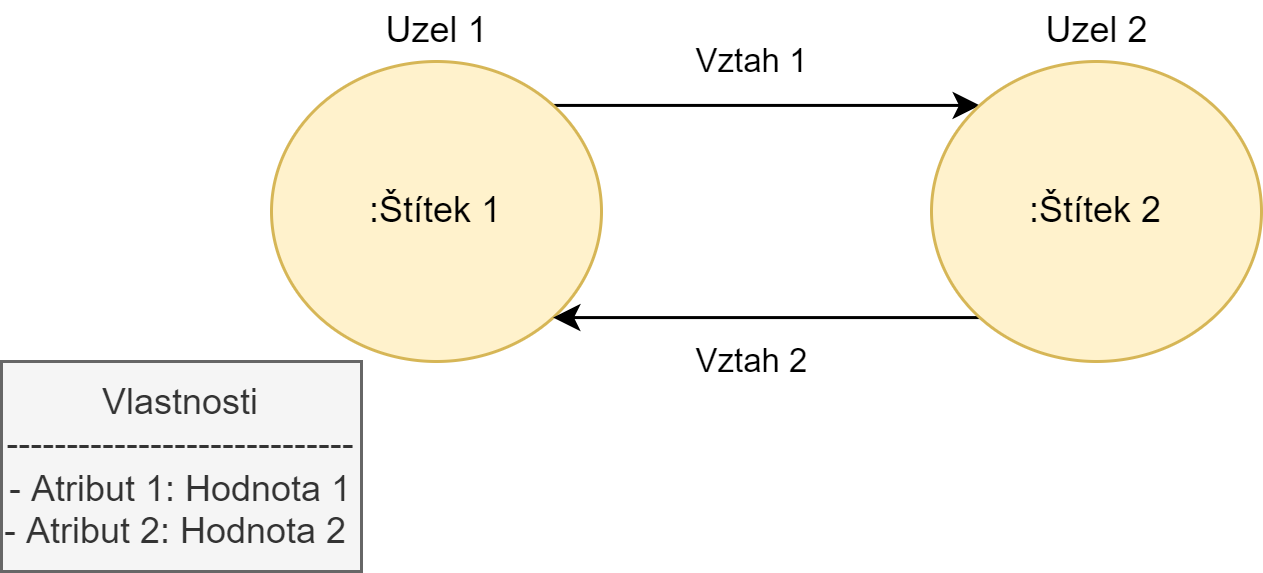
\includegraphics[width=11cm]{img/databaze/graph_components}
	\caption{Komponenty grafu.}
	\label{fig:graph_components}
	\end{figure}
\begin{itemize}
\item \textbf{Uzel} - Uzel je jeden ze dvou fundamentálních komponent který vytváří graf. Uzly slouží k reprezentaci entit nebo jiných doménových komponent.
\item \textbf{Vztah} - Vztah propojuje dva uzly a dovoluje nám vyhledávat související uzly. Uzel, ze kterého vztah začíná, se jmenuje zdrojový, zatímco uzel, ve kterém vztah končí, se nazývá cílový (šipka ukazuje směr vztahu). Vztahy musí mít vždy jen jeden zdrojový a jeden cílový uzel, proto při mazání uzlů se mažou i všechny jeho závislosti (vstupující a vystupující vztahy).
\item \textbf{Štítek} - Štítek slouží k zařazování uzlů do skupin. Všechny uzly, které jsou označené stejným štítkem, patří do jedné skupiny. Uzel může obsahovat libovolné množství štítků (0 až nekonečno). Při vyhledávání může databáze pracovat nejen s celým grafem, ale i s množinou uzlů patřící do jedné skupiny.
\item \textbf{Vlastnosti} - Vlasnost je množina dvojic klíč - hodnota, které lze ukládat s každým uzlem a vztahem. Jsou podporovány skoro všechny datové typy.
\end{itemize}

\subsubsection{Výhody}
Výhody grafové databáze jsou \cite{advantages_graph}:
\begin{itemize}
\item Struktury jsou flexibilní a přizpůsobivé.
\item Reprezentace vztahů mezi entitami je zřetelné.
\item Dotazy poskytují výsledky v reálném čase. Rychlost závisí na počtu relací.
\end{itemize}

\subsubsection{Nevýhody}
Nevýhody grafové databáze jsou \cite{advantages_graph}:
\begin{itemize}
\item Neexistuje žádný standardizovaný jazyk. Jazyk závisí na použité platformě.
\item Grafy jsou nevhodné pro transakční systémy.
\item Je těžké najít podporu, protože uživatelská základna je velice malá.
\end{itemize}

\subsection{Databáze dokumentů}
Databáze dokumentů jsou typem NoSQL databáze a  jsou navržené pro ukládání, načítání a správu informací orientovaných na dokumenty. Typické příklady jsou: MongoDB, Amazon DocumentDB, Elasticsearch. Ukázku dokumentové databáze lze vidět na obrázku č. \ref{fig:db_img_document}.
	\begin{figure}[H]
	\centering
	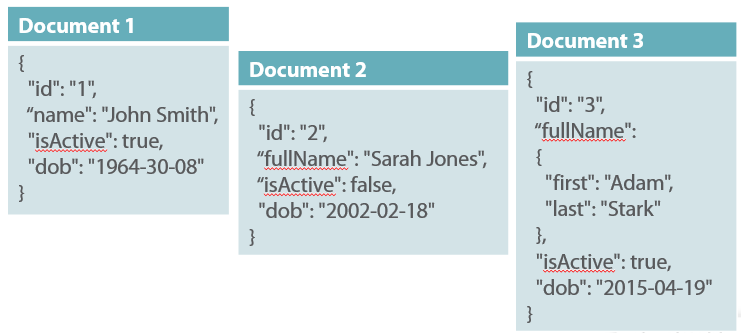
\includegraphics[width=11cm]{img/databaze/document_db}
	\caption{Ukázka dokumentově orientované databáze \cite{relat_vs_nosql}.}
	\label{fig:db_img_document}
	\end{figure}
\subsubsection{Datový model}
Základním prvkem dokumentové databáze je \textbf{Dokument}. Definice dokumentů se liší podle konkrétní implementace databáze, ale jedno mají společné: dokumenty kódují zapouzdřená data či informace do nějakého standardního formátu nebo kódování. Mezi typy kódování patří například \gls{JSON}, \gls{XML}. Dokument nemusí dodržovat pevně definovanou strukturu, takže v databázi mohou existovat dva dokumenty stejného formátu s rozdílnou strukturou dat \cite{data_model_document}.

\subsubsection{Výhody}
Výhody dokumentové databáze jsou \cite{advantages_document}:
\begin{itemize}
\item \textbf{Bez schématu} - Neexistují zde žádná omezení ve formátu a struktuře ukládání dat, proto lze bez problémů uchovávat data i ve stále se měnícím systému s obrovským množstvím dat.
\item \textbf{Údržba} - Po vytvoření dokumentu je vyžadována minimální údržba.
\item \textbf{Nezávislost dokumentů} - Dokumenty na sobě jsou nezávislé kvůli absenci cizích klíčů.
\item \textbf{Otevřené formáty} - K popisu dokumentů lze použít například formát \gls{XML}, \gls{JSON} a mnoho dalších.
\item \textbf{Věstavěné verzování} - Díky verzování lze snižovat konflikty.
\end{itemize}

\subsubsection{Nevýhody}
Nevýhody dokumentové databáze jsou \cite{advantages_document}:
\begin{itemize}
\item \textbf{Kontrola konzistence} - Je zde omezená kontrola konzistence, takže se v databázi můžou vyskytovat duplikáty.
\item \textbf{Neexistence atomicity} - V případě úpravy, která ovlivňuje dvě kolekce, je potřeba spustit dva samostatné dotazy (jeden pro každou kolekci).
\end{itemize}

\section{Existující řešení} \label{sec:existujici_reseni}
Pro vybrané typy databáze existují mnoho databázových řešení, které lze zmínit. V této kapitole se budeme zabývat především těmi nejznámějšími pro daný typ databáze, a které jsou zdarma ke stažení a používání. Pro každý typ databáze bylo vybráno vždy jedno z nejznámějších řešení.
\subsection{MySQL}
MySQL je multiplatformní databáze uplatňující relační databázový model. Komunikace s databází (získávání dat, vytváření objektů, ...) probíhá pomocí jazyka \gls{SQL}, který je rozšířen o nové funkce. Nejnovější verze MySQL je open-source, což znamená, že kdokoliv může používat a libovolně upravovat MySQL systém, aniž by musel cokoliv platit. V případě změny zdrojových kódů je potřeba nastudovat podmínky užívání definované licencí \gls{GPL} \cite{mysql}.
\newline
\indent Od samých počátků bylo MySQL optimalizováno především na rychlost i za cenu některých zjednodušení (například způsob zálohování dat). Díky tomuto lze provozovat jednoduché servery na počítači společně s jinýma aplikacema, případně jiné databáze. Server lze nakonfigurovat tím způsobem, že může využívat veškerou paměť, procesorový čas i vstupně výstupní kapacity.
\newline

\noindent MySQL server může být využit dvěma způsoby:
\begin{itemize}
\item \textbf{Klient / server} - Vícevláknový \gls{SQL} server, který podporuje různé back-endy, několik různých klientských programů a knihoven a mnoho dalšího.
\item \textbf{Věstavěná knihovna} - Vícevláknová věstavěná knihovna, kterou lze propojit do své aplikace a získat tím menší, rychlejší a snadněji spravovatelný samostatný produkt.
\end{itemize}
\subsection{PostgreSQL}
PostgreSQL je open-source objektově-relační databázový systém, který vznikl spojením relačního a objektově-orientovaného databázového systému. PostgreSQL je velice silný nástroj, který používá rozšíření jazyka \gls{SQL} společně s mnoha funkcemi, které bezpečně skladují a škálují většinu nejsložitějších datových úloh.
\newline
\indent PostgreSQL přichází s mnoha funkcemi, které jsou zaměřené na pomoc vývojářům při vytváření aplikací, správu a bezpečnost dat a odolnost proti chybám v systému. Jako další výhody lze zmínit velkou rozšiřitelnost (lze tvořit vlastní datové typy a funkce), psaní kódu v jiných programovacích jazycích, podpora \gls{ACID} a možnost provozovat server na všech hlavních operačních systémech \cite{postgres}.
\newline

\noindent PostgreSQL obsahuje mnoho funkcí, které může uživatel využít. Zde je výpis pouze část z nich:
\begin{itemize}
\item \textbf{Datové typy} - Primitivní (číslo, text, ...),  strukturované (datum, pole, ...), dokumenty (\gls{JSON}, \gls{XML}, ...), geometrie (bod, kruh, ...) a vlastní datové typy.
\item \textbf{Celistvost dat} - Unikátní hodnoty, primární a cizí klíče, zámky.
\item \textbf{Výkonnost} - Indexování pomocí stromů, výrazů. Základní a vnořené transakce.
\item \textbf{Zabezpečení} - Vícefaktorová autentikace s certifikáty, sloupcové a řádkové zabezpečení.
\item \textbf{Textové vyhledávání} - Full-textové vyhledávání.
\end{itemize}

\subsection{LevelDB}
LevelDB je open-source databáze typu Klíč-hodnota, která se používá hlavně u malých přenosných aplikací a nepotřebují žádné \gls{API} (rozhraní). Databáze byla vytvořena dvěma programátory Googlu, kteří byli inspirování již existující databází Bigtable (databáze typu klíč-hodnota, která je součástí platformy Google Cloud), ale chtěli vytvořit jednoduchou, lehce přenosnou databázi, kterou lze distribuovat zároveň s aplikací, která ji využívá.
\newline
\indent Algoritmus pro ukládání databáze funguje tak, že dočasně ukládá data v \textit{MemTable} (mezipaměť pro zpětný zápis řádků, ve které lze hledat pomocí klíče), ze které se data postupně přesouvají do \textit{SSTable} (Sorted String Table), což je tabulka seřazených řetězců, které nelze měnit. Neměnná data jsou ukládána na disk, který může být sdílen s více clustery \cite{leveldb}.
\newline

\noindent Výhody LevelDB jsou:
\begin{itemize}
\item \textbf{Jednoduché operace} - LevelDB má tři základní jednoduché operace \textit{Get} (vrací hodnotu podle klíče), \textit{Put} (vkládá dvojici klíč-hodnota) a \textit{Delete} (mazání dvojice klíč-hodnota).
\item \textbf{Bytové pole} - Klíče a hodnoty lze ukládat i do bytového pole, což může být užitečné v případě, kdy nechceme ukládat hodnoty jako řetězce.
\item \textbf{Atomické operace} - LevelDB podporuje atomické operace, to znamená, že lze použít více operací najednou v jednom nepřerušeném volání.
\end{itemize}

\subsection{MongoDB}
MongoDB je dokumentově-orientovaná databáze, která se používá zejména tam, kde je potřeba uchovávat velké množství dat. Firma MongoDB.Inc poskytuje oficiální ovladače ke všem populárním programovacím jazykům jako je například C\#, Java, C++ a mnoho dalších. Existují i neoficiální ovladače vytvořené komunitou, které pokrývají ještě více programovacích jazyků.
\newline
\indent MongoDB je vlastně ve skutečnosti server, který umožňuje vytvářet a udržovat několik databází najednou. Každá databáze může mít své vlastní kolekce, které sdružují dokumenty.  MongoDB podporuje vnořená data, což umožňuje vytvářet složité vztahy mezi dokumenty a ukládat je do stejného dokumentu, což činí práci a načítání dat extrémně efektivní ve srovnání s SQL.\cite{mongo}
\newline

\noindent Výhody MongoDB jsou \cite{advantages_mongo}:
\begin{itemize}
\item Dokumenty lze mapovat na objekty v kódu aplikace, takže se s nimi dá jednodušeji pracovat.
\item Indexování, shlukování v reálném čase a ad-hoc dotazy poskytují velice výkonné způsoby přístupu k datům a jejich analýzy.
\item MongoDB nabízí vysokou dostupnost, horizontální škálování a geografickou distribuci a to díky tomu, že je ve svém jádře distribuovanou databází.
\end{itemize}

\subsection{Neo4j}
Neo4j je open-source nativní grafová databáze, která efektivně implementuje vlastnosti grafového modelu až na úroveň úložiště, které je velmi výkonné. Pomocí Neo4j lze naimplementovat každý graf, který dokážeme nakreslit na tabuli, za pomoci ukazatelů. Stejně jako pro MongoDB, i zde existují ovladače pro populární programovací jazyky, jako například Java, .NET a mnoho dalších.
\newline
\indent Neo4j je velice populární právě z důvodu konstantních časových přechodů ve velkých grafech jak pro prohledávání do šířky, tak i do hloubky, díky efektivní reprezentaci a škálování uzlů a vztahů mezi nimi. Databáze navíc umožňuje vytvářet flexibilní schéma vlastností grafu, které se může v průběhu času přizpůsobovat, díky čemuž lze přidávat nové vztahy pro vytváření zkratek mezi uzly pro zrychlení práce s daty. Neo4j také poskytuje úplné databázové charakteristiky, které zahrnují i \gls{ACID} vlastnosti, podpory clusterů a převzetí služeb při selhání za běhu \cite{neo4j}.

\section{Jazyky} \label{sec:jazyky}
Databázové jazyky, jinak známé jako dotazovací jazyky, jsou klasifikací programovacích jazyků, které se používají k definování a přístupu k databázím. Pomocí těchto jazyků dokáže uživatel získávat nebo spravovat data v databázích. V dnešní době se jazyky (například \gls{SQL}) mohou skládat ze čtyř podjazyků, kdy každý slouží k jinému účelu v rámci vykonávání příkazů \cite{indeedDBLanguage, begginersBookDBLanguage}:
\begin{itemize}
\item \textbf{Data definition language} (DDL) - DDL umí vytvářet jednotlivé komponenty databázového schématu (tabulky, soubory, indexy, ...), které tvoří strukturu reprezentující organizaci dat v databázi. Dostupné příkazy pro jazyk DDL:
	\begin{itemize}
	\item \textbf{CREATE} - Vytvoření nového objektu (tabulka, index, ...).
	\item \textbf{ALTER} - Změna struktury objektu.
	\item \textbf{DROP} - Smazání objektu.
	\item \textbf{RENAME} - Změna názvu objektu.
	\item \textbf{TRUNCATE} - Smazání podobjektů v objektu (například záznamy v tabulce).
	\end{itemize}
\item \textbf{Data manipulation language} (DML) - DML slouží pro manipulaci s daty, které se nachází v již existující databázi. Dostupné příkazy pro jazyk DML:
	\begin{itemize}
	\item \textbf{SELECT} - Získání záznamů (dat) z tabulky.
	\item \textbf{INSERT} - Vložení nového záznamu (dat) do tabulky.
	\item \textbf{UPDATE} - Úprava existujícího záznamu v tabulce.
	\item \textbf{DELETE} - Smazání záznamu z tabulky.
	\end{itemize}
\item \textbf{Data control language} (DCL) - Pomocí DCL lze kontrolovat přístupy a práva k datům, které jsou uloženy v databázi. Uživateli lze nastavit práva k jednotlivým DML příkazům nad tabulkama / procedurama (například uživatel bude mít přístup pouze k příkazu SELECT nad tabulkou "TABULKA"). Dostupné příkazy pro jazyk DCL:
	\begin{itemize}
	\item \textbf{GRANT} - Přidání práv uživateli nad danou tabulkou / procedurou. 
	\item \textbf{REVOKE} - Odebrání práv uživateli nad danou tabulkou / procedurou.
	\end{itemize}

\item \textbf{Transaction control language} (TCL) - TCL spravuje transakce v databázi. Transakce obsahuje jeden či více DML příkazů nad tabulkama, které se vykonávají po sobě. Všechny příkazy musí být úspěšně provedeny, aby bylo možné transakci označit za úspěšnou. Ukázka jedné transakce viz obrázek č. \ref{fig:tcl_savepoint}. Dostupné příkazy pro jazyk TCL:
	\begin{itemize}
	\item \textbf{COMMIT} - Potvrzení transakce, změny provedené v transakci jsou permanentní a nejdou vzít zpět.
	\item \textbf{ROLLBACK} - Vezme zpět veškerou práci v aktuální transakci. Lze se vrátit na začátek transakce nebo k SAVEPOINTu.
	\item \textbf{SAVEPOINT} - Nastavení bodu v transakci, ke kterému se lze v budoucnu vrátit pomocí ROLLBACK.
	\end{itemize}
\end{itemize}
	\begin{figure}[H]
	\centering
	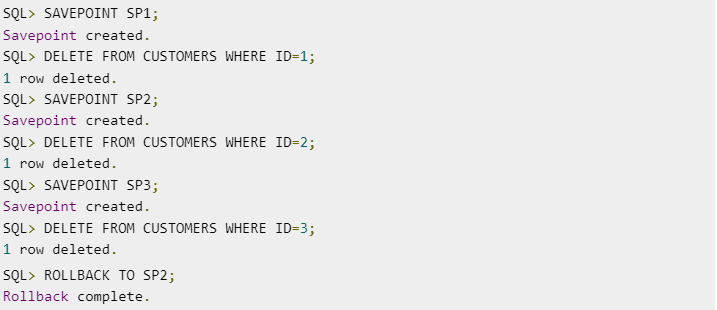
\includegraphics[width=14cm]{img/databaze/tcl_savepoint}
	\caption{Ukázka jedné transakce (bez commitu)}
	\label{fig:tcl_savepoint}
	\end{figure}

\noindent Níže v kapitolách jsou popsány příklady dnešních jazyků.
\subsection{Structured Query Language}
Structured Query Language (\gls{SQL}) je jazyk pro komunikaci s databázema, v dnešní době standard pro relační databázové systémy. Pomocí \gls{SQL} příkazů lze například vytvářet nové objekty v databázi, upravovat existující data v tabulkách nebo vytvářet různá integritní omezení a triggery. Většina existujících databázových systémů používá upravený \gls{SQL} jazyk, který navíc obsahuje dodatečná rozšíření pro splnění požadavků v jejich systémech.

\subsubsection{Syntax}
Syntaxe \gls{SQL} se skládá z unikátního seznamu pravidel a směrnic. Při psaní příkazů zde nehraje roli citlivost písma (příkazy select a SELECT jsou záměnné). Dotazy lze psát na jednu nebo více řádek, které musí / můžou být zakončené středníkem (záleží na pravidlech používaného systému). Na obrázku č. \ref{fig:sql} lze vidět příklad dotazu, který získá jména a příjmení uživatelů z tabulky 'user' s datem narození po roce 2000.
	\begin{figure}[H]
	\centering
	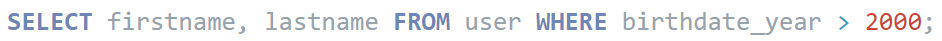
\includegraphics[width=13cm]{img/databaze/sql}
	\caption{Příklad \gls{SQL} dotazu.}
	\label{fig:sql}
	\end{figure}

\noindent Dotazy lze zanořovat do sebe, kdy výsledek jednoho dotazu jde použit jako podmínka pro druhý dotaz, viz obrázek č. \ref{fig:sql2}.
	\begin{figure}[H]
	\centering
	
\includegraphics[width=14cm]{img/databaze/sql2}
	\caption{Příklad zanořeného \gls{SQL} dotazu.}
	\label{fig:sql2}
	\end{figure}

\subsection{MongoDB Query Language}
MongoDB Query Language (\gls{MQL}) je jazyk pro získávání dat z MongoDB dokumentových databází. Dotazy zde poskytují jednoduchost v procesu načítání dat z databáze, stejně jako tomu je u \gls{SQL}. Při provádění dotazů lze také použít kritéria nebo podmínky, kterými lze načíst konkrétní data z databáze. Jazyk také podporuje \gls{CRUD} operace. Výsledky můžeme třídit, seskupovat, fitrovat a spočítat jejich četnost za pomoci agregační pipeline (zřetězeného zpracování). \gls{MQL} podporuje transakce více dokumentů \cite{mongo_lang}.

\subsubsection{Syntax}
Syntaxe \gls{MQL} je intuitivní a jednoduchá na používání i pro velice složité dotazy, protože ta samá syntaxe se používá i pro uložené dokumenty v databázi. Příklad syntaxe pro vytváření, čtení, úpravu a mazání dokumentů (\gls{CRUD}) lze vidět na obrázku č. \ref{fig:crud}.
	\begin{figure}[H]
	\centering
	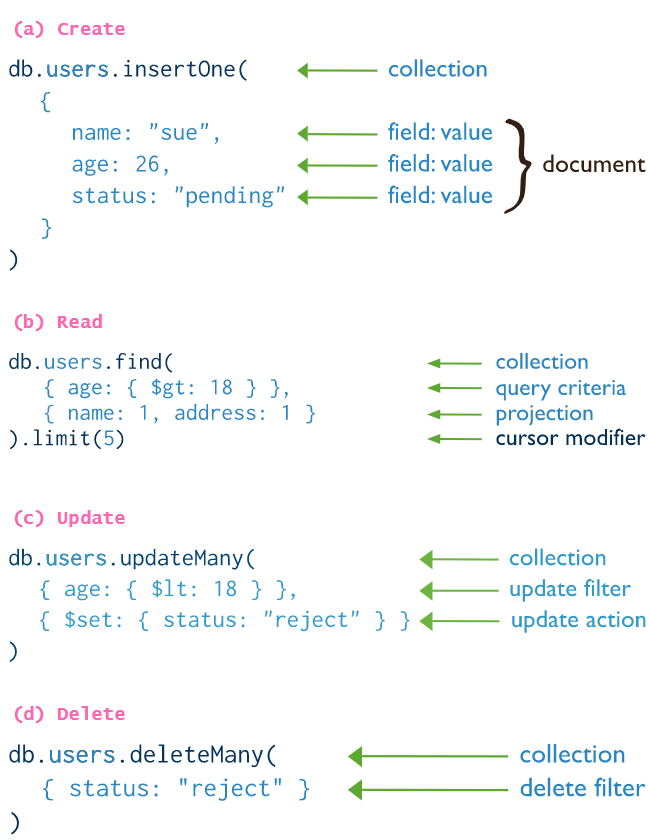
\includegraphics[width=12cm]{img/databaze/crud}
	\caption{Příklady \gls{CRUD} operací v MongoDB \cite{mongo_query}.}
	\label{fig:crud}
	\end{figure}

\subsection{Cypher Query Language}
Cypher je dotazovací jazyk pro grafovou databázi Neo4j a umožňuje získávat data z grafů. Tento jazyk byl inspirován hlavně \gls{SQL} - uživatel se zaměřuje pouze na to, jaká data chce získat, ne jak je má získat. Cypher je unikátní v tom, že poskytuje vizuální způsob, jak sladit vzory a vztahy \cite{cypher}.

\subsubsection{Syntax}
Cypher využívá \gls{ASCII}-art typ syntaxe, což je umění, které pracuje s počítačovým textem jako s výtvarným médiem (například obrázky se skládají ze znaků kódu \gls{ASCII}). Syntaxi lze vidět na obrázku č. \ref{fig:cypher_syntax}. Pro jednotlivé uzly se používají kruhové závorky, pro vztah se používá šipka s hranatýma závorkama obsahující vztah prvního uzlu s druhým uzlem.
	\begin{figure}[H]
	\centering
	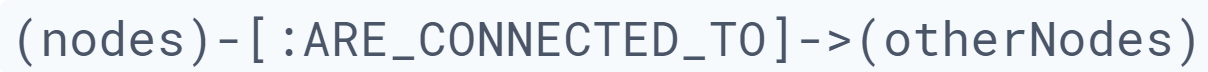
\includegraphics[width=14cm]{img/databaze/cypher_syntax1}
	\caption{Syntaxe jazyka Cypher.}
	\label{fig:cypher_syntax}
	\end{figure}
\noindent Na obrázku č. \ref{fig:cypher_sample} lze vidět jednoduchý dotaz, který hledá výsledný uzel pro vstupní uzel, kterým je člověk se jménem 'Dan', a vztahu 'LOVES' mezi uzly.
	\begin{figure}[H]
	\centering
	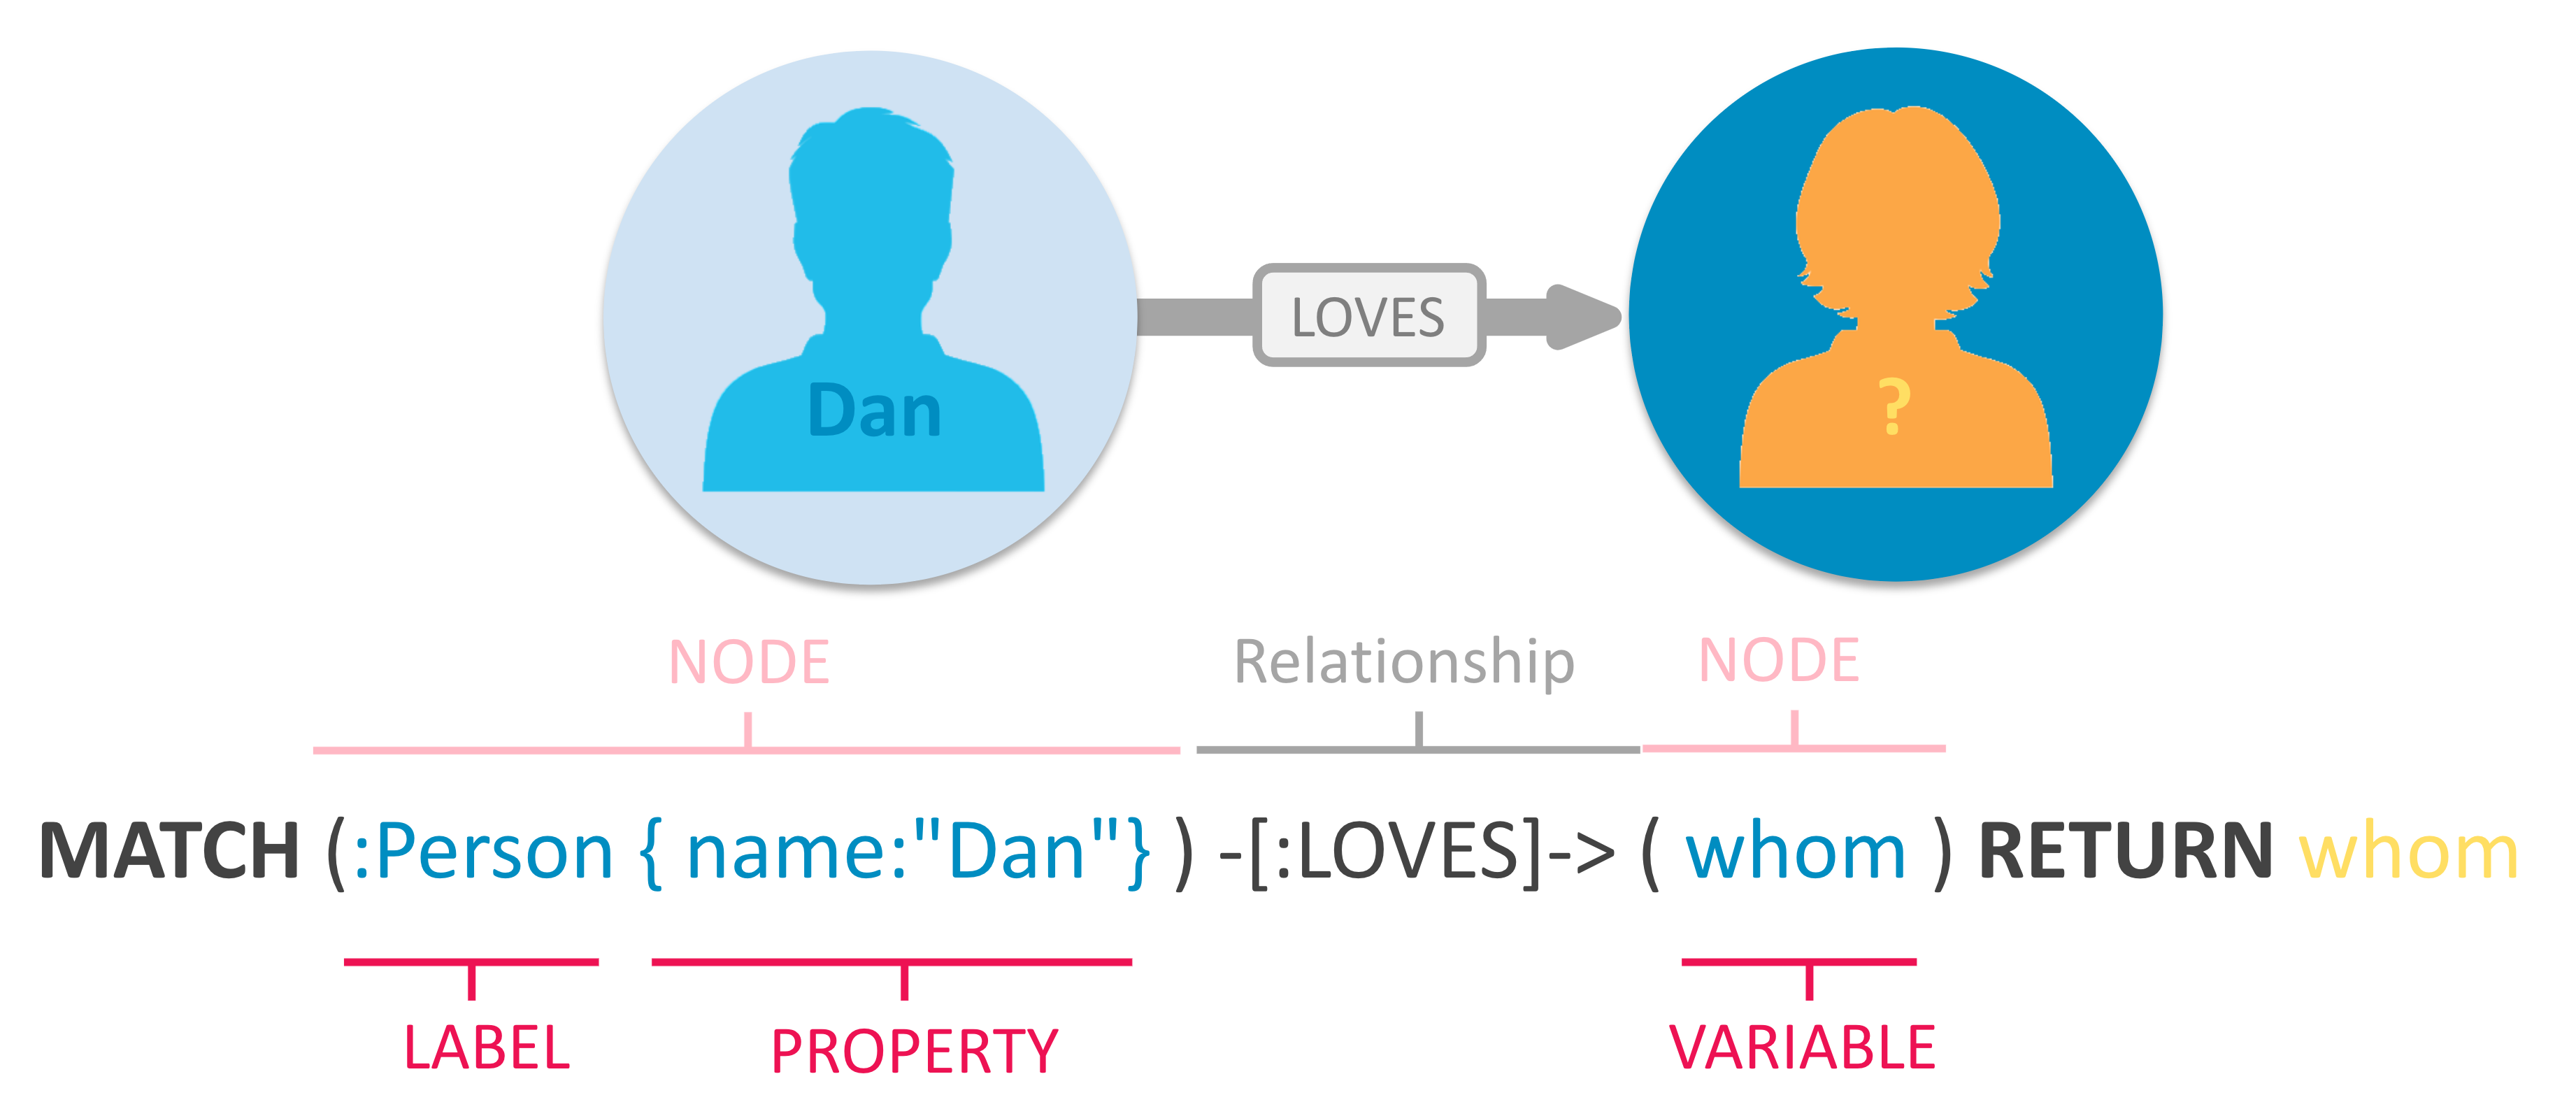
\includegraphics[width=14cm]{img/databaze/sample-cypher}
	\caption{Dotaz v jazyce Cypher \cite{cypher}.}
	\label{fig:cypher_sample}
	\end{figure}